\documentclass{article}[a4paper]
\usepackage[a4paper, total={6.5in, 9in}]{geometry}
\usepackage{float}
\usepackage{amsmath}
\usepackage{amssymb}
\usepackage{enumitem}
\usepackage{tabularray}
\usepackage{charter}
\usepackage{xcolor}
\usepackage{graphicx}
\usepackage{listings}
\usepackage{tikz}
\usepackage{parskip}
\usepackage[hidelinks]{hyperref}

\newcommand{\extlink}{
	
\begin{tikzpicture}[scale=0.1]
		\draw[rounded corners=0.5mm, line width=0.9pt] (-1, -1) rectangle (1, 1);
		\fill[white] (0, 0) rectangle (1.3, 1.3);
		\draw[line width=0.9pt, line cap=round] (0.15, 0.15) -- (1.3, 1.3);
		\draw[line width=0.9pt, line cap=round] (0.5, 1.3) -- (1.3, 1.3) -- (1.3, 0.5);
	\end{tikzpicture}
}

\lstset{
	language=Matlab,
	basicstyle=\ttfamily,
	keywordstyle=\color{blue},
	commentstyle=\color{gray},
	stringstyle=\color{red},
	showstringspaces=false,
	columns=fullflexible,
	breaklines=true,
	captionpos=b,
	backgroundcolor=\color[rgb]{0.96,0.96,0.96},
	xleftmargin=6pt,
	frame=tlbr,
	framesep=6pt,
	framerule=1pt,
}

\title{
	\huge{\textbf{
		Assignment 01
	}}\\
	\large{\phantom{}}\\
	\large{
		submitted for
	}\\
	\Large{
		\textbf{EN3551 - Digital Signal Processing}
	}\\
	\large{
		Department of Electronic and Telecommunication Engineering
	}
	\\
	\large{University of Moratuwa}
}

\author{
	\textbf{Udugamasooriya P. H. J.}\\
	220658U\\
	\small{Progress on \href{https://github.com/pulasthi-u/en3150-assignment01}{GitHub \extlink}}
}

\date{12 September 2025}

\begin{document}
	\maketitle
	
	\section{Harmonic Detection}
	
	\textbf{Question 03} Five subsets of the provided signal were formed as described. The magnitude plots of the DFTs of each of these subsets are indicated in Figure \ref{subset_dfts}.
	
	\begin{figure}[H]
		\centering
		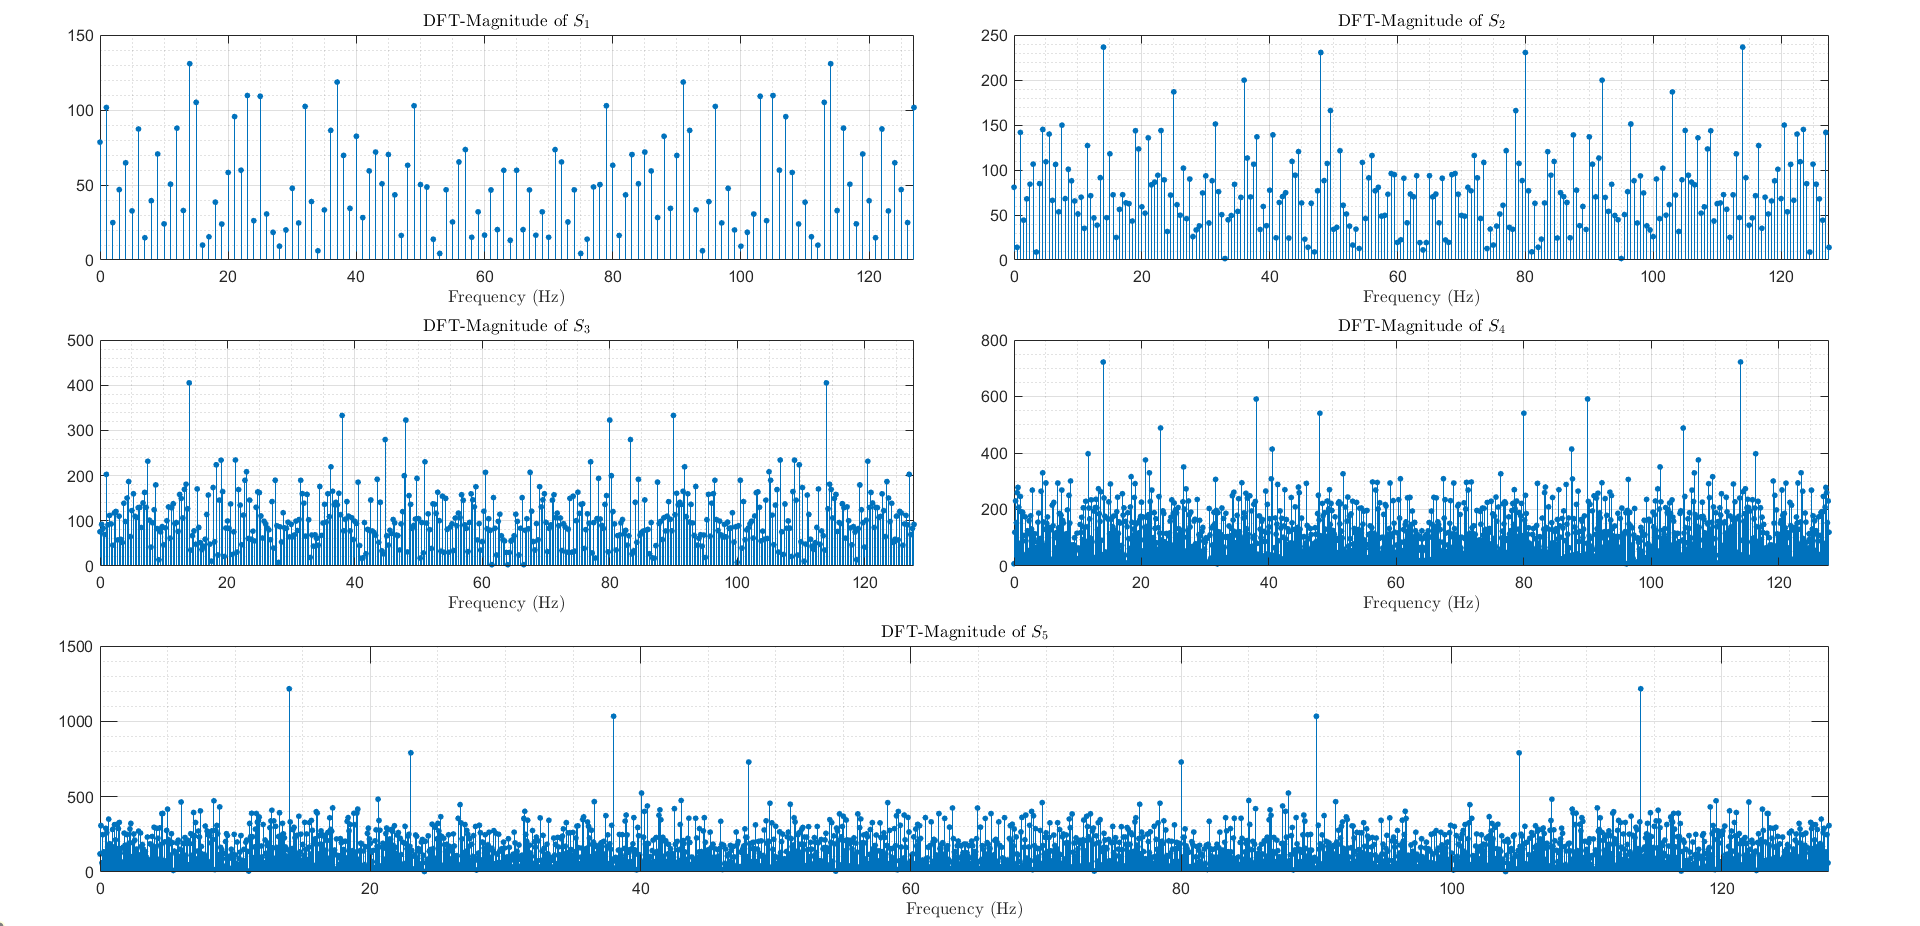
\includegraphics[width=\linewidth]{images/q1_3_1.png}
		\caption{DFT-magnitude plots of signals $S_1$ through $S_5$}
		\label{subset_dfts}
	\end{figure}
	
	\textbf{Question 04} We use this code. Figure \ref{avg_dft} shows the magnitude plot resulting from averaging the DFTs of $L = 14$ consecutive subsets taken from the given signal.
	
	\begin{figure}[H]
		\centering
		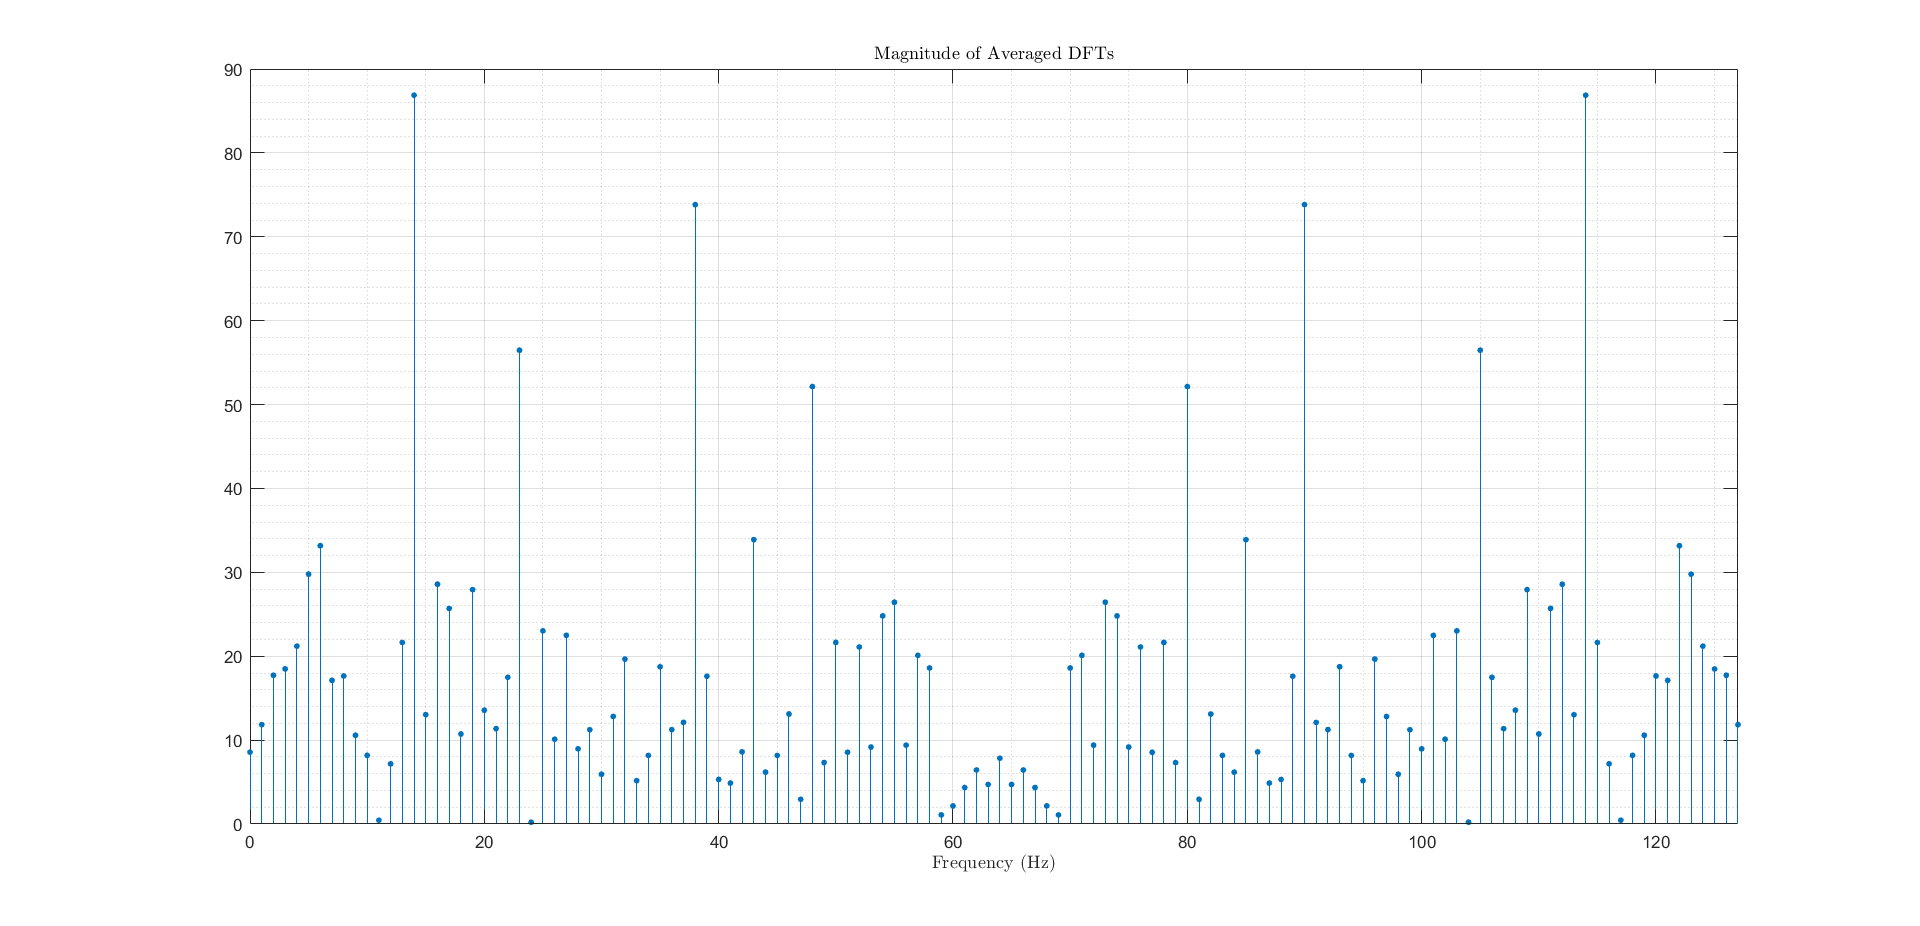
\includegraphics[width=\linewidth]{images/q1_3_2.png}
		\caption{Magnitude plot of the averaged DFT over several subsets}
		\label{avg_dft}
	\end{figure} 
	
	\section{Interpolation}
	
	\textbf{Question 01} A plot of the first 50 samples of the loaded signal is given in Figure \ref{orig_x1}.
	
	\begin{figure}[H]
		\centering
		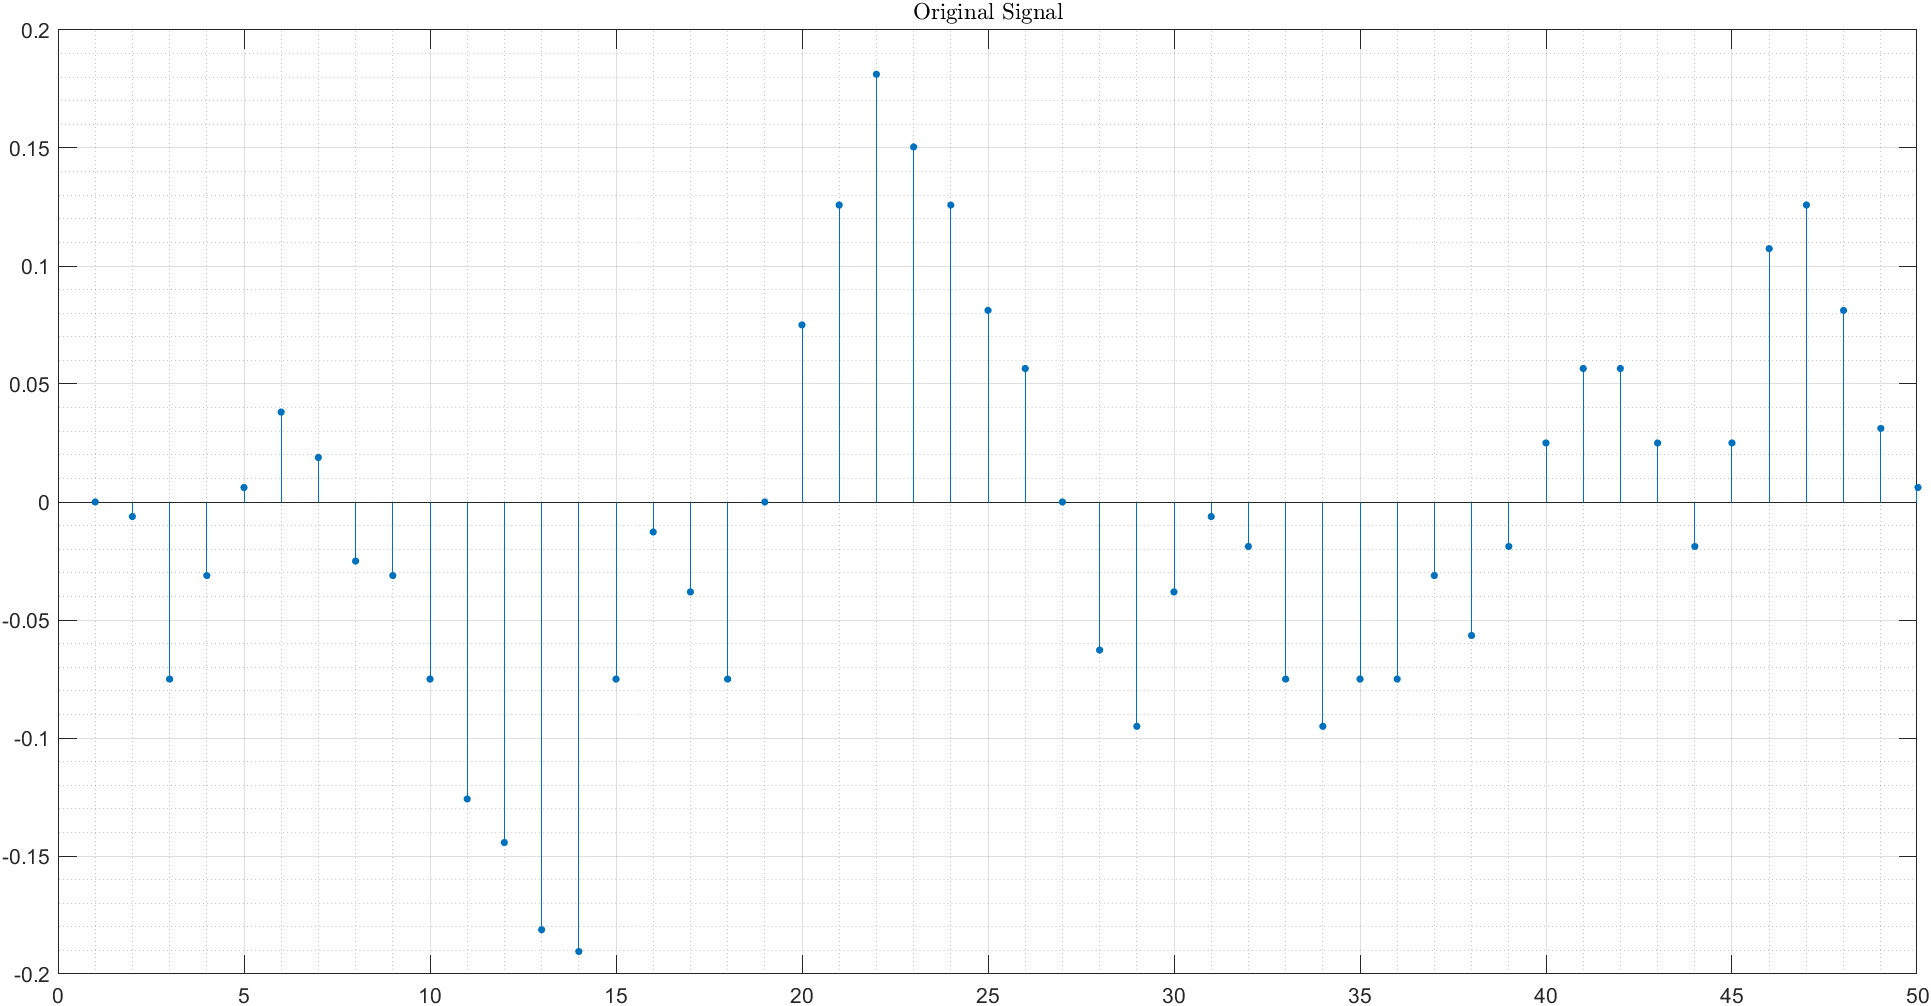
\includegraphics[width=0.9\linewidth]{images/q2_orig_sig.png}
		\caption{Original signal}
		\label{orig_x1}
	\end{figure}
	
	\textbf{Question 03} Steps (a) through (c) were carried out using the code in Listing X in Appendix \ref{code}. Outputs obtained from the code and relevant plots are as shown in Figures X, Y, and Z respectively. An analysis of the results obtained follows.
	
	\begin{enumerate}[label=(\alph*)]
		\item \phantom{a}
		\begin{figure}[H]
			\centering
			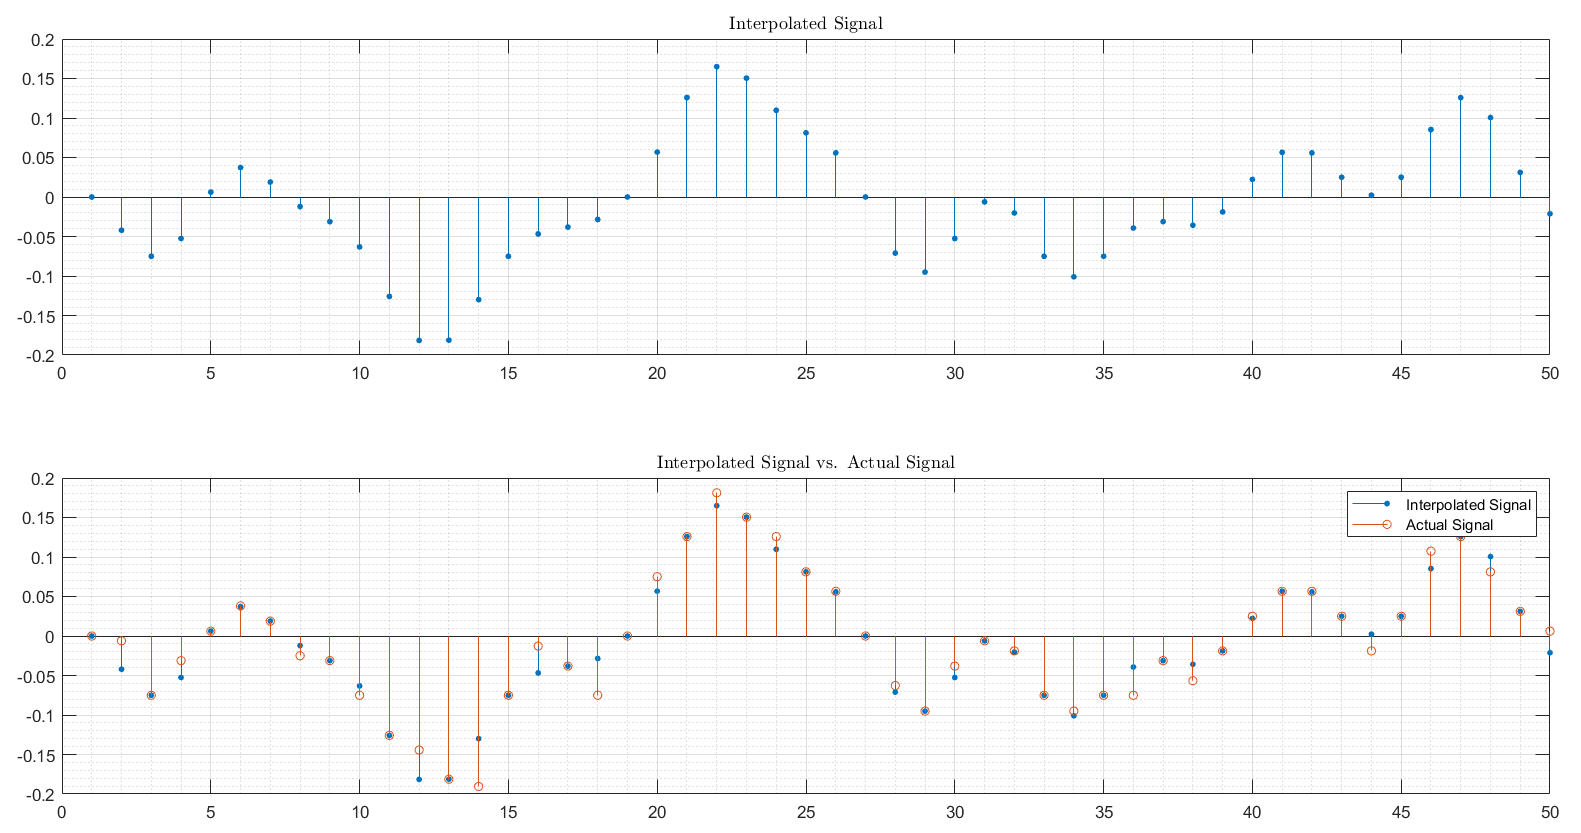
\includegraphics[width=0.9\textwidth]{images/q2_x2_interp.png}
			\caption{$x_2$ Interpolated}
			\label{x2_interp}
		\end{figure}
		
		\begin{lstlisting}[caption={abc}]
Norm of difference: 6.1447
		\end{lstlisting}
		
		\item b
		\item c
		\item d
	\end{enumerate}
	
	\appendix
	\section{Code Snippets}
	\label{code}
	
	\subsection{Harmonic Detection}
	
	\subsection{Interpolation}
	
\end{document}